% -------------- brute force popin detection ------

\section{Pop-in detection}
The pop-in effect is a reaction of the crystalline structure to load. Defects of the crystalline structure occur during loading, these then reveal themselves as discontinuous jumps in the depth at constant
load. The critical load values are characteristic for the given orientation of the given material and can be compared to theoretical predictions based on the knowledge of the crystal lattice.

\begin{figure}[ht]
  \centering
  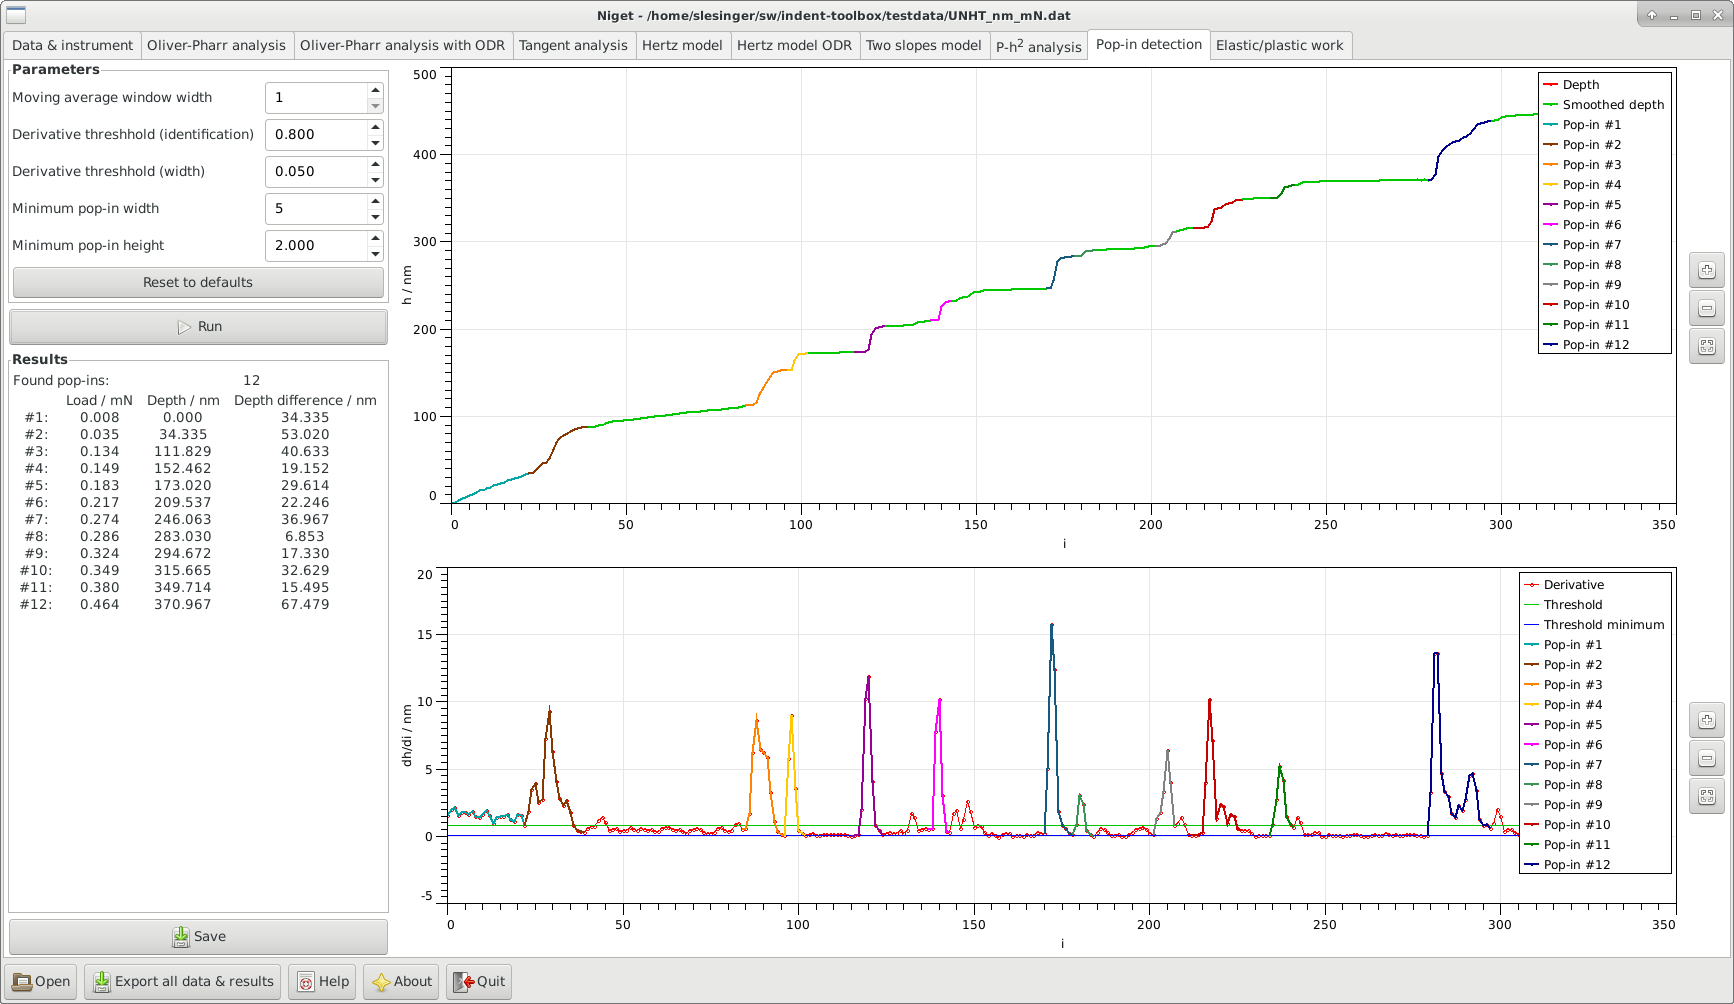
\includegraphics[width=\textwidth]{images/screen-popins}
  \caption{Pop-in detection}
\end{figure}

\subsection{Window}
The window consists of several blocks:
\begin{itemize}
 \item \emph{Info} displays the maximum depth and force during the indentation
 \item \emph{Parameters} allows the user to set the following parameters and the selected range in nm. 
        \begin{itemize}
          \item[-] \emph{Moving average window width} the width of the moving average window. The value 1 corresponds to no smoothing.
          \item[-] \emph{Derivative threshold for pop-in detection} the minimum derivative to identify the point as a pop-in.
          \item[-] \emph{Derivative threshold for pop-in width} determines how far to extend the pop-in once it was identified.
          \item[-] \emph{Minimum pop-in width} minimum number of datapoints needed for a pop-in.
          \item[-] \emph{Minimum pop-in height} (in nm) minimum jump in height needed for a pop-in.
        \end{itemize}
        These values are saved in settings. Default values are provided, but most likely the user will have to find proper values for each curve. For a detailed description see \ref{popin_calc}
       
  \item \emph{Run}  perform calculation and display curve, see section \ref{popin_calc}. 
  \emph{Results} displays the found pop-in events, the load and depth at which they occurred and the jump in the depth associated with it, see section \ref{popin_calc}.
 \item \emph{Save} save parameters and results to given file. 
 \item \emph{Graph}  
    \begin{itemize} \item[] Top: display the loading curve and the smoothed curve. 
       \item[] Bottom: display the derivative of the depth with respect to the index (pseudo-time) together with the two derivative thresholds.
  \end{itemize}
  Identified pop-ins are shown in color. \\
  Stepwise zooming/unzooming can be performed by selecting a range with the mouse and pressing the \emph{Zoom}/ \emph{Unzoom} buttons. 
		     The graph is restored to its original size by the \emph{Restore} button. Zooming in the two graphs is independent.
\end{itemize}

\subsection{Procedure} \label{popin_calc}
There is no standardized procedure how to define pop-in events. We use here a brute force direct method. %\marginpar{vysvetlujici graf}
\begin{enumerate}
 \item 
We use a moving average with a fixed width and constant weight. This means we substitute a value with its average with $s$ values to the left and to the right, $w = 2s + 1$ 
$$
\hat{x} _i = \frac1w \sum_{j = -s}^{s} x_{i+j}.
$$
The value $w = 1$ corresponds to the original data. 
Increasing the value of $w$ noise becomes less influential but important small effects can get lost as well. 
Therefore, the value should not be too large, below 11 is recommended.
\item Calculate the derivative of the loading curve with respect to the index (pseudo-time). This is the numerical derivative (in this case threee point derivative with equal steps) 
$$
dx_i = \frac12(x_{i+1} - x_{i-1}), 
$$
where $h$ is the step in the data.
\item Find the indices $i$ for which $x_i$ is larger then the \emph{Derivative threshold for pop-in detection}
\item Group the indices found in the previous step into consecutive groups.
\item Enlarge each group of indices to the left and to the right to include all values larger than \emph{Derivative threshold for pop-in width}.
\item For each group, check that the difference between the leftmost and righmost index is at least \emph{Minimum pop-in width}.
\item For each group, check that the difference in depth between the leftmost and righmost point  is at least \emph{Minimum pop-in height}.
\item For each group, find the average load for the range between leftmost and rightmost, the depth at the leftmost point (beginning of the pop-in), the difference in height between the leftmost and rightmost point and the indices.
\end{enumerate}


